\documentclass{masterthesis}

\usepackage{hyperref} % links
\usepackage{graphicx}
\usepackage{amsmath}
\usepackage{amssymb}
\usepackage{qcircuit}
\usepackage{braket}
\usepackage{float}
\usepackage[toc,page]{appendix}
\usepackage{listings}

\begin{document}

\title{Mathematical Modeling of Quantum Repeaters Chains}

\author{Lorenzo La Corte}

\advisor{}

\examiner{}

\maketitle

\chapter*{Mathematical Background}

\section*{Convolution}

Convolution is a fundamental mathematical operation used to combine two functions to produce a third function, which represents how the shape of one function is modified by the other. 

For two discrete functions \(a\) and \(b\), the convolution \(a * b\) is defined as:

\begin{equation}
    (a * b)(z) = \sum_{x=0}^{z} a(x) \cdot b(z - x)
\end{equation}

\paragraph*{Convolution of two Probability Distributions}
In the context of probability distributions, if \(X\) and \(Y\) are independent random variables with probability distribution functions \(p_X\) and \(p_Y\), their sum \(Z = X + Y\) has a probability distribution function \(p_Z\) given by the convolution of \(p_X\) and \(p_Y\):
\begin{equation}\label{eq:convolution}
    p_Z(z) = \sum_{x=0}^{z} p_X(x) \cdot p_Y(z - x)
\end{equation}

Thus, convolution is used to determine the probability distribution of the sum of independent random variables by combining their individual probability distributions.

\paragraph*{Example} 

Consider this simple example. Let $X$ and $Y$ discrete independent random variables. 

The probability distribution $\Pr(Z = z)$ of the random variable $Z = X + Y$ is computed as follows:
\begin{equation*}
    \begin{array}{|c|c|c|c|c|c|c|}
        \hline
        x & \Pr(X = x) & y & \Pr(Y = y) & z & \Pr(Z = z) & \text{Derivation of }\Pr(Z = z)\\
        \hline
        0 & 0.2 & 0 & 0.3 & 0 & 0.06 & 0.2 \cdot 0.3 \\
        \hline
        1 & 0.5 & 1 & 0.4 & 1 & 0.23 & 0.2 \cdot 0.4 + 0.5 \cdot 0.3 \\
        \hline
        2 & 0.3 & 2 & 0.3 & 2 & 0.35 & 0.2 \cdot 0.3 + 0.5 \cdot 0.4 + 0.3 \cdot 0.3 \\
        \hline
         &  &  &  & 3 & 0.27 & 0.5 \cdot 0.3 + 0.3 \cdot 0.4 \\
        \hline
         &  &  &  & 4 & 0.09 & 0.3 \cdot 0.3 \\
        \hline
    \end{array}
\end{equation*}

Note that $\Pr(Z = z)$ has five elements (all the possible sums), and it is valid as its probabilities sum to 1.

\begin{samepage}\label{page:convolution_associativity}
    The convolution operator \( * \) is associative, meaning that for any three functions \(a\), \(b\), and \(c\):
    \begin{equation}
        (a * b) * c = a * (b * c)
    \end{equation}        
\end{samepage}

\section*{Random Variables}

In this section, we fix notation on random variables and operations on them. 

Most random variables in the context of quantum repeaters
\begin{itemize}
    \item are discrete,
    \item have as domain a subset of nonnegative integers.
\end{itemize}

\paragraph*{PDF}\label{paragraph:pdf}
Let $X$ be such a random variable, then its probability distribution function is a map
\begin{equation}
    p_X : x \mapsto \Pr(X = x)
\end{equation} 
which describes the probability that its outcome will be $x \in \{0, 1, 2, \ldots \}$.

\paragraph*{CDF}\label{paragraph:cdf}
Equivalently, $X$ is described by its cumulative distribution function
\begin{equation}
    \Pr(X \leq x) = \sum_{y=0}^{x} \Pr(X = y),
\end{equation}

which is transformed to the probability distribution function as 
\begin{equation}
    \Pr(X = x) = \Pr(X \leq x) - \Pr(X \leq x - 1).
\end{equation}

\paragraph*{Independent Random Variables}\label{paragraph:independent_random_variables}
Two random variables $X$ and $Y$ are independent if 
\begin{equation}
    \Pr(X = x \text{ and } Y = y) = \Pr(X = x) \cdot \Pr(Y = y)
\end{equation}
for all $x$ and $y$ in the domain.

\paragraph*{Copies of a Random Variable}\label{paragraph:copies_of_a_random_variable}
By a \textit{copy} of $X$, we mean a fresh random variable which is independent from $X$ and identically distributed (i.i.d.).
We will denote a copy by a superscript in parentheses. For example, $X^{(1)}$, $X^{(142)}$ and $X^{(A)}$ are all copies of $X$.

The mean of $X$ is denoted by 
\begin{equation}\label{eq:expectation}
    E[X] = \sum_{x=0}^{\infty} \Pr(X = x) \cdot x
\end{equation}

and can equivalently be computed as 
\begin{equation}
    E[X] = \sum_{x=1}^{\infty} \Pr(X \geq x).
\end{equation}

\paragraph*{Function of Random Variables}\label{paragraph:function_of_random_variables}
If $f$ is a function which takes two nonnegative integers as input, then the random variable $f(X, Y)$ has probability distribution function defined as

\begin{equation}
    \Pr(f(X, Y) = z) := \sum_{\substack{x=0, y=0 \\ f(x,y)=z}}^{\infty} \Pr(X = x \text{ and } Y = y).
\end{equation}

\paragraph*{Sum of Random Variables}\label{paragraph:sum_of_random_variables}
An example of such a function is addition. 

Define $Z := X+Y$ where $X$ and $Y$ are independent, then the probability distribution $p_Z$ of $Z$ is given by 
\begin{equation}
    p_Z(z) = \Pr(Z = z) = \sum_{\substack{x=0, y=0 \\ x+y=z}}^{\infty} \Pr(X = x \text{ and } Y = y).
\end{equation}

But since $y = z - x$ this is equivalent to
\begin{align}
    p_Z(z) = \Pr(Z = z) &= \sum_{\substack{x=0}}^{z} \Pr(X = x \text{ and } Y = z - x) \\ 
                        &= \sum_{\substack{x=0}}^{z} \Pr(X = x) \cdot Pr(Y = z - x) \\
                        &= \sum_{x=0}^{z} p_X(x) \cdot p_Y (z - x)
\end{align}
which is the convolution of the distributions $p_X$ and $p_Y$, denoted as $p_Z = p_X * p_Y$ \hyperref[eq:convolution]{(see convolution)}.

Since convolution operator $*$ is associative, writing $a * b * c$ is well-defined, for functions $a$, $b$, $c$ from the nonnegative integers to the real numbers \hyperref[page:convolution_associativity]{(see associativity of convolution)}.

In general, \textbf{the probability distribution of sums of independent random variables equals the convolutions of their individual probability distribution functions}.

\section*{Geometric Distribution}\label{section:geometric_distribution}

The Geometric Distribution is a discrete probability distribution that models the number of trials needed to achieve the first success in a sequence of independent Bernoulli trials, each with the same success probability \( p \).

\subsection*{Probability Distribution Function (PDF)}\label{subsection:geometric_pdf}

The Probability Distribution Function (PDF) of a Geometric Distribution gives the probability that the first success occurs on the \( t \)-th trial. It is defined as:
\begin{equation}
    \Pr(T = t) = p (1 - p)^{t-1} \quad \text{for} \quad t \in \{1, 2, 3, \ldots \},
\end{equation}
where:
\begin{itemize}
    \item $T$ is the random variable representing the trial number of the first success,
    \item $p$ is the probability of success on each trial,
    \item $(1 - p)$ is the probability of failure on each trial.
\end{itemize}

This formula expresses that the first \( t-1 \) trials must be failures (each occurring with probability \( 1 - p \)), and the \( t \)-th trial must be a success (with probability \( p \)).

\subsection*{Cumulative Distribution Function (CDF)}\label{subsection:geometric_cdf}

The Cumulative Distribution Function (CDF) of a Geometric Distribution gives the probability that the first success occurs on or before the \( t \)-th trial. It is defined as:
\begin{equation}
    \Pr(T \leq t) = 1 - (1 - p)^t.
\end{equation}

\paragraph*{Derivation of the CDF}

This is the derivation of the CDF of a Geometric Distribution, from its PDF
\begin{align*}
    \Pr(T \leq t) &= 1 - \Pr(T > t) \\
    &= 1 - \sum_{k=t+1} \Pr(T = k) \\
    &= 1 - \left\{p (1 - p)^t + p (1 - p)^{t+1} + p (1 - p)^{t+2} + \ldots\right\} \\
    &= 1 - p (1 - p)^t \sum_{k=0} (1 - p)^k \\
    &= 1 - (1 - p)^t \sum_{k=0} p (1 - p)^k \\
    &= 1 - (1 - p)^t.
\end{align*} % tocheck

This CDF formula indicates the probability that the first success occurs within the first \( t \) trials.

\chapter*{Mathematical Model for \\ Waiting Time and Fidelity}

We derive expressions for the waiting time and fidelity of the first generated end-to-end link in the repeater chain protocol. 

We derive a recursive definition for the random variable $T_n$, which \textbf{represents the waiting time in a $2n$-segment repeater chain}.

Extending this definition to the Werner parameter $W_n$ of the pair, which stands in one-to-one correspondence to its fidelity $F_n$ using the equation:
\begin{equation}
    F_n = \frac{1 + 3 W_n}{4}.
\end{equation}

Note that all operations in the repeater chain protocols we study
\begin{itemize}
    \item Entanglement generation over a single hop
    \item Distillation
    \item Swapping
\end{itemize}
take a duration that is a multiple of ${L_0}/{c}$, the time to send information over a single segment.

For this reason, it is common to denote the waiting time in \textbf{discrete units} of ${L_0}/{c}$, which is a convention we comply with for $T_n$. Cutoffs as well follow the same discrete units. % tocheck

\newpage
\section*{Heraldeld Entanglement Generation}

\subsection*{Waiting Time for Elementary Entanglement}
In modeling the random variable $T_n$, which represents the waiting time in a $2^n$ segment repeater chain, we can reason by induction.

The base case \textbf{$T_0$ is the waiting time for the generation of elementary entanglement}.

Since we model the generation of single-hop entanglement by attempts which succeed with a fixed probability $p_{\text{gen}}$, the waiting time $T_0$ is a discrete random variable (in units of $L_0 /c$) which follows a \hyperref[section:geometric_distribution]{geometric distribution} with probability distribution given by 
\begin{equation}
    \Pr(T_0 = t) = p_{\text{gen}} (1 - p_{\text{gen}})^{t-1} \quad \text{for} \quad t \in \{1, 2, 3, \ldots \}.
\end{equation}

% tocheck: is it really more convenient to specify T_0 by its CDF? I think in David paper is not like this
For what follows, it will be more convenient to specify $T_0$ by its \hyperref[subsection:geometric_cdf]{cumulative distribution function} (CDF), which is given by
\begin{equation}
    \Pr(T_0 \leq t) = 1 - (1 - p_{\text{gen}})^t.
\end{equation}

\begin{figure}[h]
    \centering
    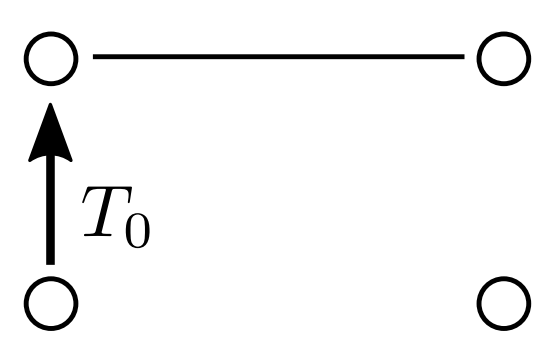
\includegraphics[width=0.2\linewidth]{images/gen.png}
    \caption{For two segments, $T_0$ represents the waiting time for the generation of a single link between two nodes without any intermediate repeater nodes.}
    \label{fig:gen}
\end{figure}


\subsection*{Werner Parameter for Elementary Entanglement}\label{subsection:werner_parameter_gen}

The output state for the generation is a Werner state with Werner parameter $w_0$. 

\subsection*{Numerical Examples}

To plot the CDF and PDF of the waiting time for the entanglement generation protocol, we can use the following code snippet:
% todo: rework the style of the code snippet
\begin{lstlisting}[language=Python]
def entanglement_generation(p_gen=0.5, t_trunc=20):
    parameters = {
        # A protocol is represented by a tuple of 0 and 1,
        # where 0 stands for swap and 1 stands for distillation.
        # This example is a 0-level swap protocol,
        # as we consider only the entanglement generation.
        "protocol": (),
        # success probability of entanglement generation
        "p_gen": p_gen,
        # truncation time for the repeater scheme.
        # It should be increased to cover more time step
        # if the success proability decreases.
        # Commercial hardware can easily handle up to t_trunc=1e5
        "t_trunc": t_trunc,
        "w0": 0.98, # ignore this for the sake of the example
        "p_swap": 0.5  # ignore this as well
    }
    pmf, _ = repeater_sim(parameters)
    return pmf
\end{lstlisting}
The following figures show the CDF and PDF of the waiting time for the entanglement generation protocol, with $p_{\text{gen}} = 0.2$ and $p_{\text{gen}} = 0.5$. We can see that the waiting time is \textbf{distributed according to a geometric distribution}, as expected.

In order for the algorithm to be computationally feasible, \textbf{the waiting time is truncated}, in this case at $t = 20$. The parameter $t_{trunc}$ in the algorithm should chosen to be large enough to capture the bulk of the distribution, but small enough to keep the computation time reasonable. The truncation brings to an approximation of the distribution, as the probability of waiting for more than 20 units of time is not considered: this is more visible in the top plot, where the CDF is less close to 1 at $t = 20$.

\begin{figure}[ht]
    \centering
    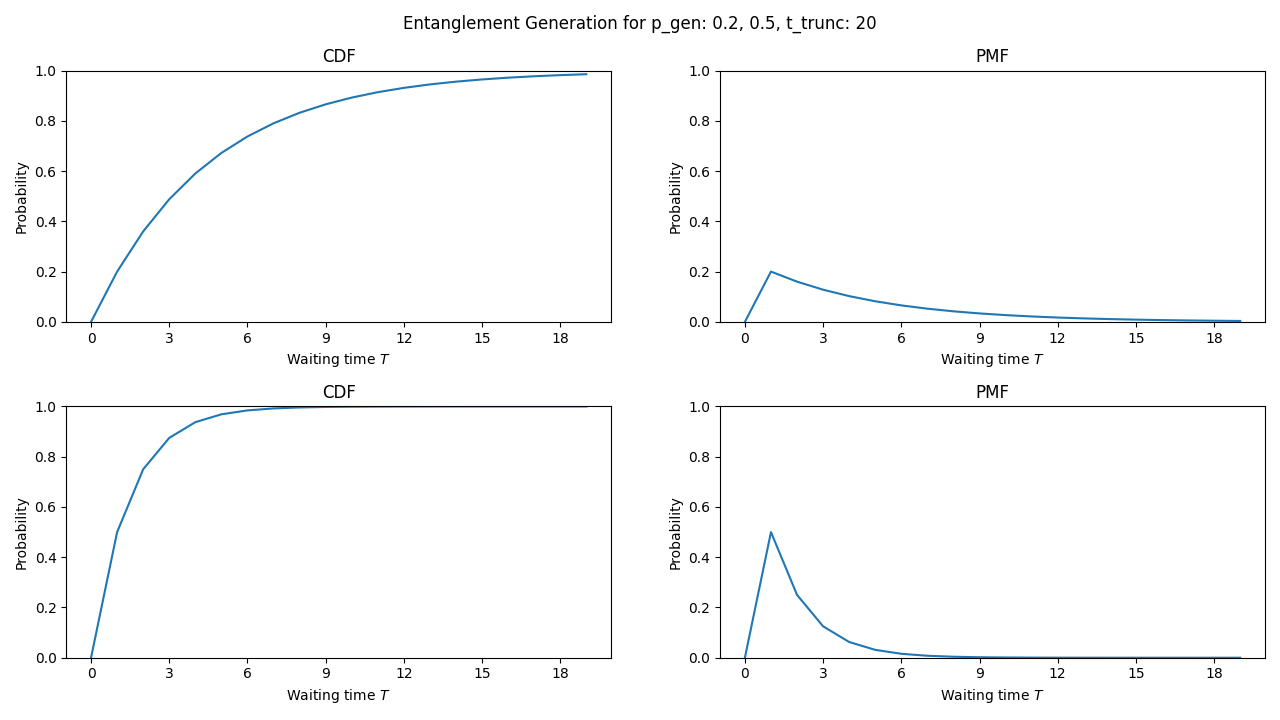
\includegraphics[width=1\linewidth]{images/gen_example_20.png}
    \caption{CDF and PDF of the waiting time for the entanglement generation protocol, with $p_{gen} = 0.2$ (top) and $p_{gen} = 0.5$ (bottom).}
\end{figure}

\newpage
\section*{Entanglement Swapping}

Once we have generated elementary entanglement, we can use it to \textbf{create entanglement over longer distances by entanglement swapping}.
We defined $T_0$ as the waiting time for the generation of elementary entanglement, and our base for the induction.
We now define our inductive step assuming that we have found an expression for $T_n$ and we want to construct $T_{n+1}$. 

In order to perform the entanglement swap to produce a single $(2^n+1)$-hop link, a node needs to wait for the production of two $(2^n)$-hop links, one on each side. 

Denote the waiting time for the pairs by $T_n^{(A)}$ and $T_n^{(B)}$, both of which are i.i.d. with $T_n$, as they are \hyperref[paragraph:copies_of_a_random_variable]{copies} of it. 

\subsection*{Waiting Time for Entanglement Swapping}

\subsubsection*{Time until both pairs are available}

We introduce a new random variable $M_n$ modeling the time until both pairs are available
\begin{equation}\label{eq:waiting_time_pair}
    M_n := g_T(T_n^{(A)} , T_n^{(B)}) .
\end{equation}

The function $g_T$ is generally defined as the maximum of the two waiting times
\begin{equation}\label{eq:waiting_time_pair_max}
    g_T(t_A, t_B) := \max(t_A, t_B).
\end{equation}
which is also \textbf{the time at which the entanglement swap ends}. 

This is distributed according to the CDF
\begin{equation}
    \Pr(M_n \leq t) = \Pr(T_n^{(A)} \leq t \text{ and } T_n^{(B)} \leq t) = \Pr(T_n \leq t) ^ 2.
\end{equation}

From it, we can derive the PDF
\begin{align}\label{eq:pdf_waiting_time_pair}
    \Pr(M_n = t) &= \sum_{\substack{t_A, t_B: \\ t = \max(t_A, t_B)}} \Pr(T_n^{(A)} = t_A \text{ and } T_n^{(B)} = t_B) .
\end{align}

% todo: add a concrete example coming from the code, with \Pr(T_n^{(A)} = t_A), \Pr(T_n^{(B)} = t_B and \Pr(M_n = t)

\subsubsection*{Number of steps required}

We introduce now $K_n$, a random variable following a \hyperref[subsection:geometric_pdf]{geometric distribution}
\begin{equation}\label{eq:pdf_swap_steps}
    \Pr(K_n = k) = p_{swap} (1 - p_{swap})^{k-1}
\end{equation}
modeling \textbf{the number of steps $k$ until the first successful swap} at level $n$.

The fact that it follows a geometric distribution is a direct consequence of our choice to model the success probability $p_{swap}$ to be independent of the state of the two input links. 

\subsubsection*{Derivation of $T_{n+1}$}
The derivation of $T_{n+1}$ requires us to combine the random variable for the number of steps required $K_n$ and the random variable for the waiting time for one attempt $M_n$.

In order to find the relation between $M_n$ and $T_{n+1}$, note that when entanglement swap fails, the two input are lost and need to be
regenerated. The regeneration of fresh entanglement after each failing entanglement swap \textbf{adds to the waiting time}. 

Thus, $T_{n+1}$ is a \textit{compound random variable}: it is the sum of $K_n$ copies of $M_n$. 

Since the number of entanglement swaps $K_n$ is geometrically distributed, we say that $T_{n+1}$ is a \textit{geometric compound sum} of $K_n$ copies of $M_n$, denoted as
\begin{equation}
    T_{n+1}=\sum_{k=1}^{K_{n}} M_{n}^{(k)}
\end{equation}

\subsubsection*{Derivation of the PDF of $T_{n+1}$}

The probability distribution of the waiting time $T_{n+1}$
\begin{align}
    \Pr(T_{n+1} = t) &= \Pr\left[\sum_{k=1}^{K_{n}} M_{n}^{(k)} = t\right] \nonumber \\
    \intertext{is computed as the marginal of the waiting time conditioned on a fixed number of swaps}
    \Pr(T_{n+1} = t) &= \sum_{k=1}^{\infty} \Pr(K_{n} = k) \cdot \Pr\left[\left( \sum_{j=1}^{k} M_{n}^{(j)} \right) = t\right].
\end{align}

Plugging in the expressions for $\Pr(K_n = k)$ \hyperref[eq:pdf_swap_steps]{(...)} and recalling that the sum of $k$ copies of $M_n$ can be expressed as a \hyperref[eq:convolution]{convolution}, we get
\begin{equation}\label{eq:pdf_waiting_time_swap}
    \Pr(T_{n+1} = t) = \sum_{k=1}^{\infty} p_{\text{swap}}(1 - p_{\text{swap}})^{k-1} \left( \ast_{j=1}^{k} m \right)
\end{equation}
where, from \ref{eq:pdf_waiting_time_pair}
\begin{equation}\label{eq:pdf_waiting_time_pair_convolution}
    m(t) := \Pr(M = t) = \sum_{\substack{t_A, t_B: \\ t = \max(t_A, t_B)}} \Pr(T_n^{(A)} = t_A \text{ and } T_n^{(B)} = t_B) .
\end{equation}

\subsection*{Werner Parameter for Entanglement Swapping}

Considering two entangled pairs, respectively with werner parameters $w_A$ and $w_B$, the output werner parameter $w_{out}$, if we do not consider decoherence, will be % todo: for the thesis, cref werner parameter
\begin{equation}
    w_{out} = w_A \cdot w_B .
\end{equation}

However, when the first of the two pairs is generated, it has to wait for the elementary generation of the other; \textbf{during this time the first generated pair decoheres}. In particular, a Werner state $\rho(w)$ residing in memory for a time $\Delta(t)$ will transform into the Werner state $\rho(w_{decayed})$ with 
\begin{equation}\label{eq:w_decayed}
    w_{\text{decayed}} = w \cdot e^{-\Delta t / T_{coh}}
\end{equation}
where $T_{coh}$ is the joint coherence time of the two quantum memories holding the qubits. % todo: for the thesis, refer to coherence time and q. memories

Denote by $A$ and $B$ the input links to the entanglement swap and denote by $\left(t_{A}, w_{A}\right)$ and $\left(t_{B}, w_{B}\right)$ their respective delivery times and Werner parameters. 
% todo: add image
Without loss of generality, suppose that the link $A$ is produced after link $B$, i.e. $t_{A} \geq t_{B}$. 

Link $A$ is produced last, so the entanglement swap will be performed directly after its generation and hence link $A$ will enter the entanglement swap with Werner parameter $w_{A}$. Link $B$ is produced earliest and will therefore decohere until production of link $A$.

It follows that $B$'s Werner parameter decoheres accordingly to (\ref{eq:w_decayed}), and therefore is, immediately before the swap, equal to
\begin{equation*}
    w_{B}^{\prime} = w_{B} \cdot e^{-\left|t_{A}-t_{B}\right| / T_{coh}} .
\end{equation*}

Thus, the entanglement swap would produce the $2^{n+1}$-hop state with Werner parameter
\begin{align}
w_{out} &= w_{A} \cdot w_{B}^{\prime} \nonumber \\
        &= w_{A} \cdot w_{B} \cdot e^{-\left|t_{A}-t_{B}\right| / T_{coh}} .
\end{align}

Notice that choosing $t_{A} > t_{B}$ would have lead to the same result.

In order to model at the same time the Werner Parameter and the Waiting Time we use a joint random variable $(T_n, W_n)$.

In the \textbf{base case}, for a single segment ($n=0$), we are in the \hyperref[subsection:werner_parameter_gen]{(already discussed)} entanglement generation phase.
Here, the \textbf{waiting time and Werner parameter are uncorrelated} because we model the attempts at generating single-hop entanglement to be independent and to each take equally long. 

At the \textbf{recursive step} $n$, we model the waiting time and Werner parameter as a joint random variable $(T_n, W_n)$.

To define it properly, we introduce the concept of \textit{forgetting sum} $\widehat{\sum}$, defined on sequences of tuples $\left\{\left(x_{j}, y_{j}\right) \mid 1 \leq j \leq m\right\}$ for some $m \in\{1,2, \ldots\}$ as
\begin{equation}
    \widehat{\sum}_{j=1}^{m}\left(x_{j}, y_{j}\right):=\left(\sum_{j=1}^{m} x_{j}, y_{m}\right) \tag{14}
\end{equation}

This notation is key to characterize the joint random variable $(T_{n+1}, W_{n+1})$, as the Werner parameter of the output link is only influenced by the links that the successful entanglement swap acted upon, as we will see in the following.

Using this concept, we define the joint random variable $(T_{n+1}, W_{n+1})$ as
\begin{equation}\label{eq:joint_random_variable}
    (T_{n+1}, W_{n+1}) := \widehat{\sum}_{k=1}^{K_n} (M_n, V_n)^{(k)}.
\end{equation}

Starting from the auxiliary variable for the output waiting time of a pair $M_n$ (\ref{eq:waiting_time_pair}), we introduce another auxiliary random variable for the Werner parameter of the output link $V_n$, which will depend on the Werner parameters of the input links. 

We define the auxiliary joint random variable $(M_n, V_n)$ as
\begin{equation}
    (M_n, V_n) := g\left((T_n, W_n)^{(A)}, (T_n, W_n)^{(B)}\right).
\end{equation}

The function $g$ is given by
\begin{equation}
    g\left((t_A, w_A),(t_B, w_B)\right) := \left(g_T(t_A, t_B), g_W\left((t_A, w_A),(t_B, w_B)\right)\right)
\end{equation}
where $g_T$ is defined in eq. \ref{eq:waiting_time_pair_max} and % todo: I wrote that is the maximum before, adapt it
\begin{equation}
    g_W\left((t_A, w_A),(t_B, w_B)\right) := w_A \cdot w_B \cdot e^{-\frac{|t_A-t_B|}{T_{\text{coh}}}}
\end{equation}
with $T_{\text{coh}}$ the quantum memory coherence time.

We already studied the expression for the waiting time $T_{n+1}$. The other random variable $W_{n+1}$ directly derives from $V_{n}$, which expresses the Werner parameter of the produced $2^{n+1}$-hop link in case the swap is successful.

To prove that $V_{n}$ is formulated properly, we argue that $g_{W}$ correctly computes the Werner parameter of the output link after an entanglement swap.

The key idea that leads to the forgetting sum in \ref{eq:joint_random_variable} is the following: if the entanglement swap fails, then the $2^{n+1}$-hop link with its Werner parameter will never be produced since both initial $2^{n}$-hop entangled pairs are lost. Thus, for the waiting time we should consider the sum of the waiting times of all the attempts, but for the Werner parameter we should only consider the last successful attempt.

Let's explain it further.

In order to find how the Werner parameter on level $n+1$ is expressed as a function of the waiting times and Werner parameters at level $n$, consider a sequence $\left(m_{j}, v_{j}\right)$ of waiting times $m_{j}$ and Werner parameters $v_{j}$, where $j$ runs from 1 to the first successful swap $k$. 
\begin{itemize}
    \item $m_{j}$ correspond to the waiting time until the end of the entanglement swap that transforms two $2^{n}$-hop links into a single $2^{n+1}$-hop link
    \item $v_{j}$ to the output link's Werner parameter if the swap were successful. 
\end{itemize}

From previus results, we found that the total waiting time is given by $\sum_{j=1}^{k} m_{j}$, the sum of the duration of the production of the lost pairs (see \ref{eq:pdf_waiting_time_swap}). 

Note, however, that the Werner parameter of the $2^{n+1}$ hop link \textbf{is only influenced by the links that the successful entanglement swap acted upon}. Since the entanglement swaps are performed until the first successful one, the output link is the last produced link and therefore its Werner parameter equals $v_{k}$. 

We thus find that the waiting time $t_{\text {final }}$ of the first $2^{n+1}$-hop link and its Werner parameter $w_{\text {final }}$ are given by:
\begin{align}
    t_{final} &= \sum_{j=1}^{k} m_{j} \\ 
    w_{final} &= v_k 
\end{align}
or, in a more compact form
\begin{equation}
    \left(t_{final}, w_{final}\right) = \left(\sum_{j=1}^{k} m_{j}, v_{k}\right) .
\end{equation}

Taking into account that the number of swaps $k$ that need to be performed until the first successful one is an instance of the random variable $K_{n}$, we arrive at the full recursive expression for the waiting time and Werner parameter at level $n+1$ as given in \ref{eq:joint_random_variable}.

\subsubsection*{Derivation of $W_{out}$}
Let's now derive the expression for the Werner parameter of the output link $W_{out}$.

Let $W_{s}(t)$ be the \textbf{average Werner parameter} of the output link of \textbf{one attempt}, given that it succeeds and finishes at time $t$
\begin{equation}
    W_s(t) = \sum_{\substack{t_A, t_B:\\ t = \max(t_A, t_B)}} \Pr(T_A = t_A, T_B = t_B) \cdot [p_{swap} \cdot w_{\text{out}}](t_A, t_B)
\end{equation}

By taking \ref{eq:joint_random_variable} and replacing the iteration over all pair of possible input Werner parameters for each $k$ by convolution we get
\begin{equation}
    W_{out} = \sum_{k=1}^{\infty} p_{swap} (1 - p_{swap})^{k-1} \left[ \left( \ast_{j=1}^{k-1} m \right) \ast \left( m \cdot W_{s} \right) \right].
\end{equation}

Where $m$ is defined in \ref{eq:pdf_waiting_time_pair_convolution}.

$W_{out}$ represents the weighted average of the Werner parameter of the output link, over all possible sequences of failed attempts, followed by a successful one:
\begin{itemize}
    \item all possible sequences of failed attempts are represented by the $k-1$ of $m$,
    \item the successful attempt is represented by the convolution of $m$ and $W_{s}$.
\end{itemize}



\subsection*{Numerical Examples}

To plot CDF, PDF and Werner parameter of the waiting time for a 3-level entanglement swapping protocol, we can use the following code snippet:
% todo: rework the style of the code snippet
\begin{lstlisting}[language=Python]

\end{lstlisting}

The Figure \ref{fig:swap} shows the CDF and PDF of the waiting time for the entanglement swapping protocol, with $p_{gen} = 0.2$, $p_{swap} = 0.2$, and $t_{trunc} = 8000$. 

The truncation approximated the distribution: the probability of waiting for more than 200 units of time is not considered. Thus, the plot only covers 98.57\% of the distribution. However, the initial bit of the Werner parameter curve is more visible using this truncation.

We can see that the Werner parameter, which measures the quality of the entanglement
\begin{itemize}
    \item starts from a value around $0.43$,
    \item immediately ($t = 8$) reaches its peak value of $0.87$,
    \item rapidly decreases, reaching a value similar to the starting one.
\end{itemize}

This is due to the fact that the entanglement is lost over time, and the longer the waiting time, the lower the quality of the entanglement.
% todo: but this doesn't explain why in the first few instant it is so low
\begin{figure}[ht]
    \centering
    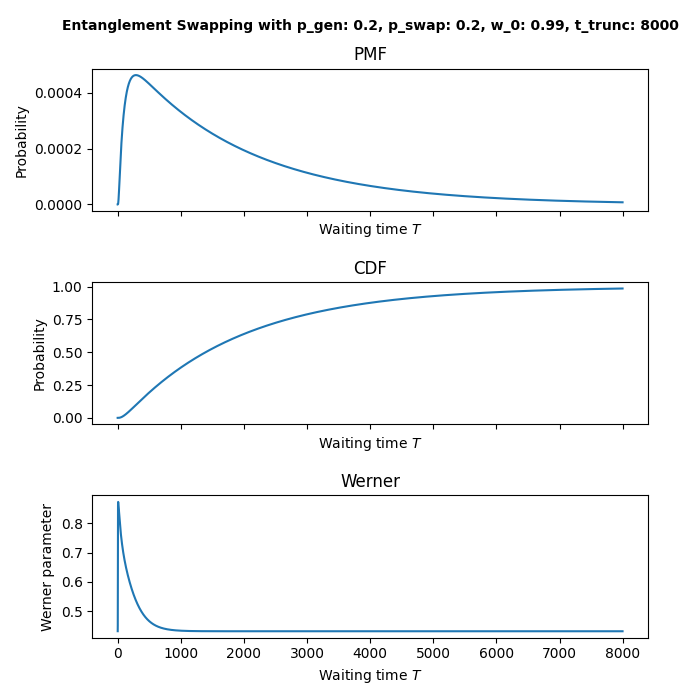
\includegraphics[width=1\linewidth]{images/swap_example_8000.png}
    \caption{CDF and PDF of the waiting time for the entanglement swapping protocol, with $p_{gen} = 0.2$, $p_{swap} = 0.2$, and $t_{trunc} = 8000$.}
    \label{fig:swap}
\end{figure}


\end{document}